\documentclass[pdftex,english,oribibl]{llncs}

%% Spracheinstellungen laden
\usepackage[english]{babel}

%% Schriftart in der Ausgabe/Eingabe
\usepackage[T1]{fontenc}
\usepackage{textcomp}
\usepackage[latin1]{inputenc}
\usepackage{enumerate}

%% Zitate
\usepackage[numbers]{natbib}
\bibliographystyle{abbrvnat}
\bibliographystyle{abnt-num}
%\bibliographystyle{dinat}
%\bibliographystyle{plainnat}
%\bibliographystyle{splncs}
%% Similar to option "sectionbib" but \refname instead of \bibname
\makeatletter
\renewcommand\bibsection{\section*{\refname\@mkboth{\MakeUppercase{\refname}}{\MakeUppercase{\refname}}}}
\makeatother

%% Index
%\usepackage{makeidx}
%\makeindex

%% PDF Einstellungen
% muss nach natbib geladen werden!
\usepackage{nameref}
\usepackage{varioref}
\usepackage[pdfusetitle,pdftex,colorlinks]{hyperref}
\hypersetup{pdfborder={0 0 0}}
\hypersetup{bookmarksdepth=3}
\hypersetup{bookmarksopen=true}
\hypersetup{bookmarksopenlevel=1}
\hypersetup{bookmarksnumbered=true}
\usepackage{color}
\hypersetup{colorlinks=false}

%\usepackage[section]{tocbibind}

\makeatletter
\gdef\@keywords{}
\def\keywords#1{\gdef\@keywords{#1}}
\gdef\@subtitle{}
\def\subtitle#1{\gdef\@subtitle{#1}}

%% modified from llncs
\renewenvironment{abstract}{%
  \list{}{\advance\topsep by0.35cm\relax\small%
          \leftmargin=1cm%
          \labelwidth=\z@%
          \listparindent=\z@%
          \itemindent\listparindent%
          \rightmargin\leftmargin}%
          \item[\hskip\labelsep\bfseries\abstractname]}{%
  \if!\@keywords!\else{\item[~]\item[\hskip\labelsep\bfseries\keywordname]\@keywords}\fi%
  \endlist}

\AtBeginDocument{%
  \if!\@subtitle!\else\hypersetup{pdfsubject={\@subtitle}}\fi
  \if!\@keywords!\else\hypersetup{pdfkeywords={\@keywords}}\fi
}
\makeatother

% llncs hyperref fix
\makeatletter
\providecommand*{\toclevel@author}{0}
\providecommand*{\toclevel@title}{0}
\makeatother

%% Grafiken
\usepackage[pdftex]{graphicx}
\DeclareGraphicsExtensions{.pdf,.jpg,.png}
\usepackage{subfigure}

%% Mathe
\usepackage{amsmath}
\usepackage{amssymb}

%% Listings
\usepackage{listings}
\lstset{escapechar=\%, frame=tb, basicstyle=\footnotesize}

%% Sonstiges
\newcommand{\TODO}[1]{\par\textcolor{red}{#1}\marginpar{\textcolor{red}{TODO}}}
\newcommand{\TODOX}[1]{\textcolor{red}{#1}\marginpar{\textcolor{red}{TODO}}}
\pagestyle{plain}

% Keine "Schusterjungen"
\clubpenalty = 10000
% Keine "Hurenkinder"
\widowpenalty = 10000 \displaywidowpenalty = 10000

%%%%%%%%%%%%%%%%%%%%%%%%%%%%%%%%%%%%%%%%%%%%%%%%%%%%%%%%%%%%%%%%%%%%%%%%%%%%%%%
%%% BEGIN DOCUMENT
%%%%%%%%%%%%%%%%%%%%%%%%%%%%%%%%%%%%%%%%%%%%%%%%%%%%%%%%%%%%%%%%%%%%%%%%%%%%%%%
\title{Security Evaluation}
% \subtitle{My (optional) Subtitle}
\author{Prince Thomas}
\institute{University of Stuttgart\\Institute of Software Technology (ISTE)\\70569 Stuttgart, Germany}


\begin{document}

\maketitle

\begin{abstract}
Software security is an idea implemented to secure software against malicious attack and other hacker risks so that the software continues to function correctly under such potential risks. Security is necessary to provide integrity, authentication and availability. The fast growth rate of software and software products makes the software security aspect even more critical. Most organizations these days want their information system to be managed as safely as possible. Security Evaluation is the basic step in achieving this goal for any organization. Security Evaluation is particularly important because of the rapidly changing environment of the information security system or the operation system. In this survey we are performing a study on Software Security Evaluation techniques. A detailed analysis of Qualitative and Quantitative Security Evaluation approaches are being carried out. The suitability and challenges of different methods of each of this approach is studied. The systems where these techniques are being used are investigated to understand the performance of security evaluation methods.\\

\textbf{Keywords:} Security, Security Evaluation, Security Metrics, Model-Based Metrics, Quantitative Security Evaluation , Qualitative Security Evaluation
\end{abstract}


\section{Introduction}

  Software security is the idea of engineering software so that it continues to function correctly under malicious attack \cite{1281254_McGraw}. The fast-growing software systems and huge amount of data handling makes the software security an important aspect in Modern software development. Measuring and assessing software security is a critical concern as it is undesirable to develop risky and insecure software. 
  
  Now a days we are hearing news about the new and new security threats every day. One such case of security threat was the phishing mail incident happened with the twitter users on the weekend of January 3, 2009, several users on the social network Web site, Twitter, became victims of a phishing attack. The users were deceived into giving away their passwords when they received an e-mail similar to one that they would receive from Twitter with a link that read, "hey, check out this funny blog about you..". The link redirects to a site misguiding as the real Twitter site. Any personal information entered by the user on the fake site is then captured by the attacker. Generally, most of security incidents are caused by software flaws and bugs called security holes and vulnerabilities. Normally a hacker tries to find and exploit security holes present in the software. He does not create security holes on his own. As a result, ensuring software security has become so critical. Software security has to be evaluated to make sure that software is minimally susceptible to threats. Evaluation of software security is so challenging because of the non-predictability of the threats and attacker behaviors. 

  In this paper a detailed survey of software security evaluation is done. First a brief description about software security metrics is presented. Then different security evaluation techniques based on qualitative and quantitative security evaluation methods are discussed. Qualitative evaluation methods identify and analyze common vulnerabilities and the probability and damage of risks are evaluated qualitatively. Quantitative evaluation methods are model based and can be described mathematically. The rest of this paper is organized as follows. Section \ref{sec:softwaremetrics} provides a brief overview of Software Security Metrics, their importance and the classifications . Section \ref{sec:qualitative} describes about the qualitative security evaluation. Section \ref{sec:quantitative} about the quantitative security evaluation and finally the paper is concluded with section \ref{sec:conclusions}.


\section{Software Security Metrics}\label{sec:softwaremetrics}
Metrics is a measurement standard which defines what is to be measured, how to be measured and helps the security practitioners to manage the product efficiently. Security metrics is the powerful tool that helps security practitioners to integrate security features into their system. The security metrics are gaining lot of significance now a days because with the help of the data obtained from them software security decisions can be taken and which in turn helps the software developers to secure their software product. 

\subsection{Importance of Software Security Metrics}
Security metrics help in decision making regarding security-related attributes of a process, system, or organization. In particular, security metrics can be applied to compare the effectiveness of different security mechanisms, or to indicate the degree to which security requirements of an organization are being met. In addition, they can also be used to systematically improve the security level of a system, or to predict this security level in a future point in time. All the people involved in the software life cycle from developers to users use the security metrics for different use cases. For example Technical Personnels(Developers) use security metrics to decide which configuration change is the most effective to increase network resilience, Management members for financial investment on security and finally end users for the trustworthiness of a software products available in the market.

The desired properties of a good security metric are granularity, availability, cost effectiveness, localization and validation \cite{8017389_Ramos}. 
\subsection{Classification of Security Metrics}
The security metrics can be classified as Fig. \ref{fig:security_metric_types}.

\begin{figure}[h]
	\centering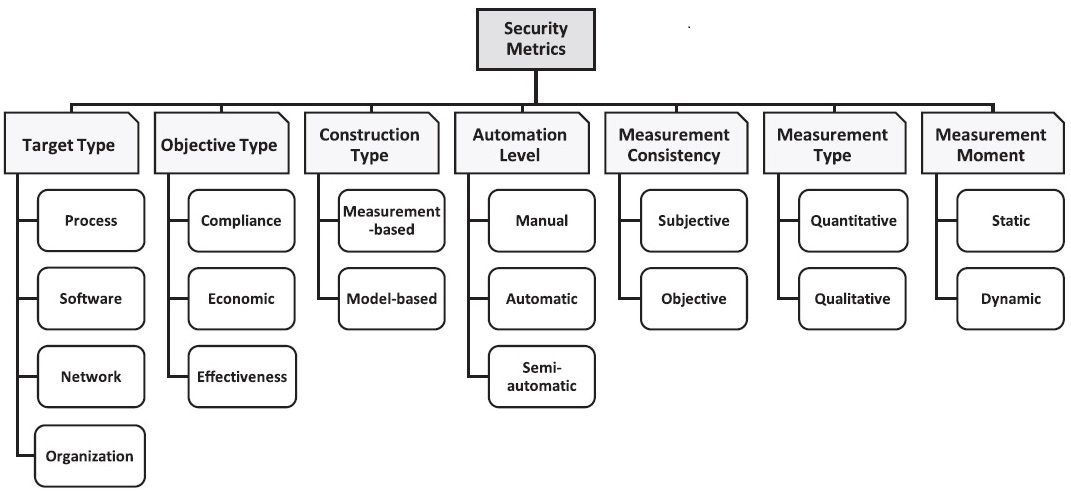
\includegraphics[width=\linewidth]{figures/security_metric_types.jpg}
	\caption{Classification of Security Metrics \cite{8017389_Ramos}.}
	\label{fig:security_metric_types}
\end{figure}

\begin{enumerate}[(a)]
	\item {\textbf{Target Type:} Security metrics can be categorized according to the target they evaluate. The most common targets assessed (and respective security metrics) are the following:}
	\begin{enumerate}[(i)]
		\item {\textbf{Process:} Process security metrics quantify the security level of a product by assessing its associated development process.}
		\item {\textbf{Software:} Software security metrics evaluate software security by assessing source code defects, software (mis)configuration, or other vulnerabilities present in software components.}
		\item {\textbf{Network:} Network Security Metrics(NSMs) assess the security of entire networks or parts thereof.}
		\item {\textbf{Organization:} Organization security metrics evaluate the physical and personnel security of an organization.}
	\end{enumerate}

	\item {\textbf{Objective Type:} Based on its objective type security metric can be classified as:}
	\begin{enumerate}[(i)]
	\item {\textbf{Compliance:} Compliance security metrics measures how well the security requirements of a target is being met based on the security methods and policies.}
	\item {\textbf{Economic:} Metrics taking into consideration of the financial aspects of security.}
	\item {\textbf{Effectiveness:} It measures how effectively the security measures can perform against security threats or violations.}
	\end{enumerate}

	\item {\textbf{Construction Type:} Based on the way security metrics is derived, they can be classified as:}
	\begin{enumerate}[(i)]
	\item {\textbf{Measurement-based:} This security metric is used to quantify the security property that is being measured.}
	\item {\textbf{Model-based:} Here the metrics values are derived from the complex mathematical equations used to define the formal mathematical model of the target. Refer Fig. \ref{fig:modelbased_metric} for a simple representation of a model-based security metric. Examples of models used to evaluate security metrics are attack graphs, Markov models, attack trees, Bayesian networks, etc. In the following sections the detailed evaluation of model-based security metrics is described.}

	\begin{figure}[h]
		\centering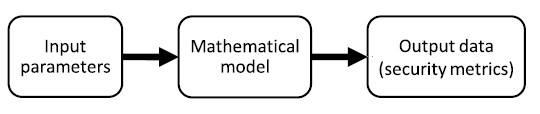
\includegraphics[width=0.5\linewidth]{figures/modelbased_metric.jpg}
		\caption{Evaluation Process of Model-Based Security Metrics \cite{8017389_Ramos}.}
		\label{fig:modelbased_metric}
	\end{figure}
	\end{enumerate}

	\item {\textbf{Automation Level:} Based on the level of automation used for the measurements the security metric can be classified as:}
	\begin{enumerate}[(i)]
	\item {\textbf{Manual:} The collection of metrics values are being carried out manually(by humans).}
	\item {\textbf{Automatic:} Metrics values are being collected with the help of computer system without the intervention of humans.}
	\item {\textbf{Semi-Automatic:} Measurement is carried out with the help of both humans and computer systems.}
	\end{enumerate}

	\item {\textbf{Measurement Consistency:} Corresponding to the consistency of the metric values, security metrics can be classified as:}
	\begin{enumerate}[(i)]
	\item {\textbf{Subjective:} Security metric is subjective to the person performing the metric measurement. Different people evaluating the same security property using same method can produce different results.}
	\item {\textbf{Objective:} Same result is being obtained irrespective of the person performing the evaluation.}
	\end{enumerate}

	\item {\textbf{Measurement Type:} According to the type of the measurement security metrics can be classified as:}
	\begin{enumerate}[(i)]
		\item {\textbf{Quantitative:} Quantitative security metrics are expressed as percentages or cardinal numbers (i.e., numbers that count something, instead of ordinal numbers, which only denote the position occupied by a given object).}
		\item {\textbf{Qualitative:} Qualitative security metrics are expressed by labels such as high-medium-low values. Ordinal numbers can also be regarded as qualitative values.}
	\end{enumerate}

	\item {\textbf{Measurement Moment:} Depending on the instance of time at which the security metrics are applied to assess a given target, they can be classified as either static or dynamic::}
	\begin{enumerate}[(i)]
	\item {\textbf{Static:} Static, or pre-deployment, security metrics are developed to be measured before the assessed target enters operation.}
	\item {\textbf{Dynamic:} Dynamic, or run-time, security metrics are those developed to be constantly measured, during the operation of the target being evaluated.}
	\end{enumerate}

\end{enumerate}
	
\section{Qualitative Security Evaluation}\label{sec:qualitative}
'Qualitative'- means "involving distinctions or involving comparisons based on qualities". Qualitative security evaluation methods identify and analyze common vulnerabilities and the probability and damage of risks are evaluated qualitatively.
\subsection{Security Patterns for Qualitative Security Evaluation}
In case of qualitative security evaluation different security patterns are evaluated for the security evaluation.  A short description of different security patterns and their objectives are described below \cite{HALKIDIS2006379}.
\begin{enumerate}[(a)]
	\item{The objective of the \textbf{Check pointed System pattern} is to organize a system so that its state can be recovered and restored to a known valid state, in case of a component failure.}
	\item{The objective of the \textbf{Standby pattern} is to organize a system so that the service provided by one component can be resumed from a different component.}
	\item{The objective of the \textbf{Comparator-Checked Fault Tolerant System pattern} is to organize a system, so that an independent failure of one component (i.e. a failure of a component that does not affect other components at all) will be detected quickly and so that an independent single-component failure will not cause a system failure.}
	\item {The objective of the \textbf{Replicated System pattern} is to organize a system that allows provision from multiple points of presence and recovery, in the case of failure of one or more components or links.}
	\item {The objective of the \textbf{Error Detection/Correction pattern} is to add redundancy to data (data replication) to facilitate later detection of and recovery of errors.}
	\item {The objective of the\textbf{ Protected System pattern} is to organize a system so that all access by clients is mediated by a guard that enforces a security policy.}
	\item{The objective of the \textbf{Policy pattern} is to isolate policy enforcement to a discrete component of an information system and to ensure that policy enforcement activities are performed in the proper sequence.}
	\item{The objective of the \textbf{Authenticator pattern} is to perform authentication of a requesting process, before deciding access to distributed objects.}
	\item{The objective of the \textbf{Subject Descriptor pattern} is to provide access to security-relevant attributes of an entity, on whose behalf operations are to be performed.}
	\item{The objective of the \textbf{Secure Communication pattern} is to ensure that mutual security policy objectives are met, when there is a need for two parties to communicate in the presence of threats.}
	\item{The objective of the \textbf{Security Context pattern} is to provide a container for security attributes and data relating to a particular execution context, process, operation or action.}
	\item{The objective of the \textbf{Security Association pattern} is to define a structure which provides each participant in a Secure Communication with the information it will use to protect messages to be transmitted to the other party.}
	\item{The objective of the \textbf{Secure Proxy pattern} is to define the relationship between the guards of two instances of Protected System, in the case when one instance is entirely contained within the other.}
\end{enumerate}

\subsection{Qualitative criteria for evaluation of security pattern}
Spyros T. Halkidis, Alexander Chatzigeorgiou and George Stephanides in their paper "A qualitative analysis of software security patterns" \cite{HALKIDIS2006379} had mentioned three set of qualitative criteria for evaluation of security pattern.The first category is based on 10 guiding principles for building secure software by Viega and McGraw (2002) \cite{GaryMcGraw2002}. The 10 principles are Secure the weakest link, Practice defense in depth, System should fail securely, Follow the principle of least privilege, Compartmentalize system, System should be simple, Promote privacy,	Remember that hiding secrets is hard, Reluctant to trust and Use community resources (well-tested solutions). The second set of criteria focuses on software development problems which can lead to software security holes and are buffer overflows, poor access control mechanisms and Race conditions.The last set of criteria can be described as how well a specific security pattern might respond to different categories of attacks as they are described by Howard and LeBlanc (2002) \cite{Howard:2002:WSC:579079}. The model purposed by Howard and LeBlanc is called \textbf{STRIDE} model. The different attacks are \textbf{S}poofing identity attacks, \textbf{T}ampering with data attacks, \textbf{R}epudiation attacks, \textbf{I}nformation disclosure attacks, \textbf{D}enial of Service (DoS) attacks and \textbf{E}levation of privilege attacks.


\subsection{Security Evaluation using Vulnerability Assessment and Penetration Testing (VAPT)}
Vulnerability assessment is the process of scanning the system or software or a network to find out the weakness and loophole in that. These loopholes can provide back-door for the  attacker to attack the victim. A system may have access control vulnerability, Boundary condition vulnerability, Input validation vulnerability, Authentication Vulnerabilities, Configuration Weakness Vulnerabilities, and Exception Handling Vulnerabilities etc. \cite{GOEL2015710}.

Penetration testing is the next step after vulnerability assessment. Penetration testing is the process of exploiting the system in an authorized manner to find out the possible exploits in the system. In penetration testing, the tester has the authority to do penetration testing and intently exploit the system and find out possible exploits. The life cycle of VAPT shown in Fig. \ref{fig:vapt_lifecycle}.

\begin{figure}[h]
	\centering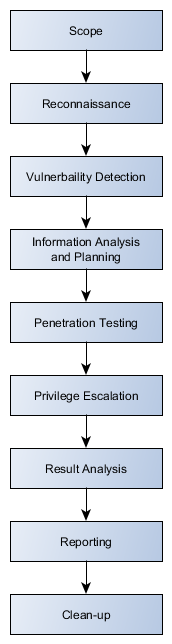
\includegraphics[width=0.2\textwidth]{figures/vapt_lifecycle.png}
	\caption{Vulnerability Assessment and Penetration Testing Life cycle \cite{GOEL2015710}.}
	\label{fig:vapt_lifecycle}
\end{figure}

The different vulnerability assessment techniques are \textbf{static analysis:} analyze the code structure and contents of the system , \textbf{manual testing:} tester uses his own knowledge and experience to find out the vulnerabilities, \textbf{automated testing:} use automated vulnerability testing tools to find out vulnerabilities in the system and \textbf{fuzz testing:} inputs invalid or any random Data into system and then look for crashes and failure.

The different Penetration testing techniques are \textbf{Black box testing:} the tester do not have prior knowledge about the network architecture or systems of the testing network, \textbf{Grey box testing:} tester has partial knowledge about the system and \textbf{White box testing:} tester has complete knowledge about the system.

There are different VAPT tools available in the market for doing VAPT assessment. Few examples are MBSA (vulnerability scanner for windows), AppScan (web vulnerability scanner for windows)and w3af (web vulnerability scanner for cross-platform).

\subsection{Case study : Evaluation of web security mechanism using vulnerability and attack Injection (VAIT)}
Here evaluation of security mechanisms in the context of web applications is described using the above mentioned qualitative security evaluation. Most common vulnerabilities in web applications was presented in a field study that classified 655 XSS and SQLi security patches of six widely used Linux, Apache, MySQL and PHP (LAMP) web applications \cite{6629992_Fronseca}. 

The typical VAIT set up for security evaluation in case of a web application is given in the Fig. \ref{fig:vait_setup}

\begin{figure}[h]
	\centering
	\subfigure[VAIT in a typical setup]{\label{fig:vait_setup}
		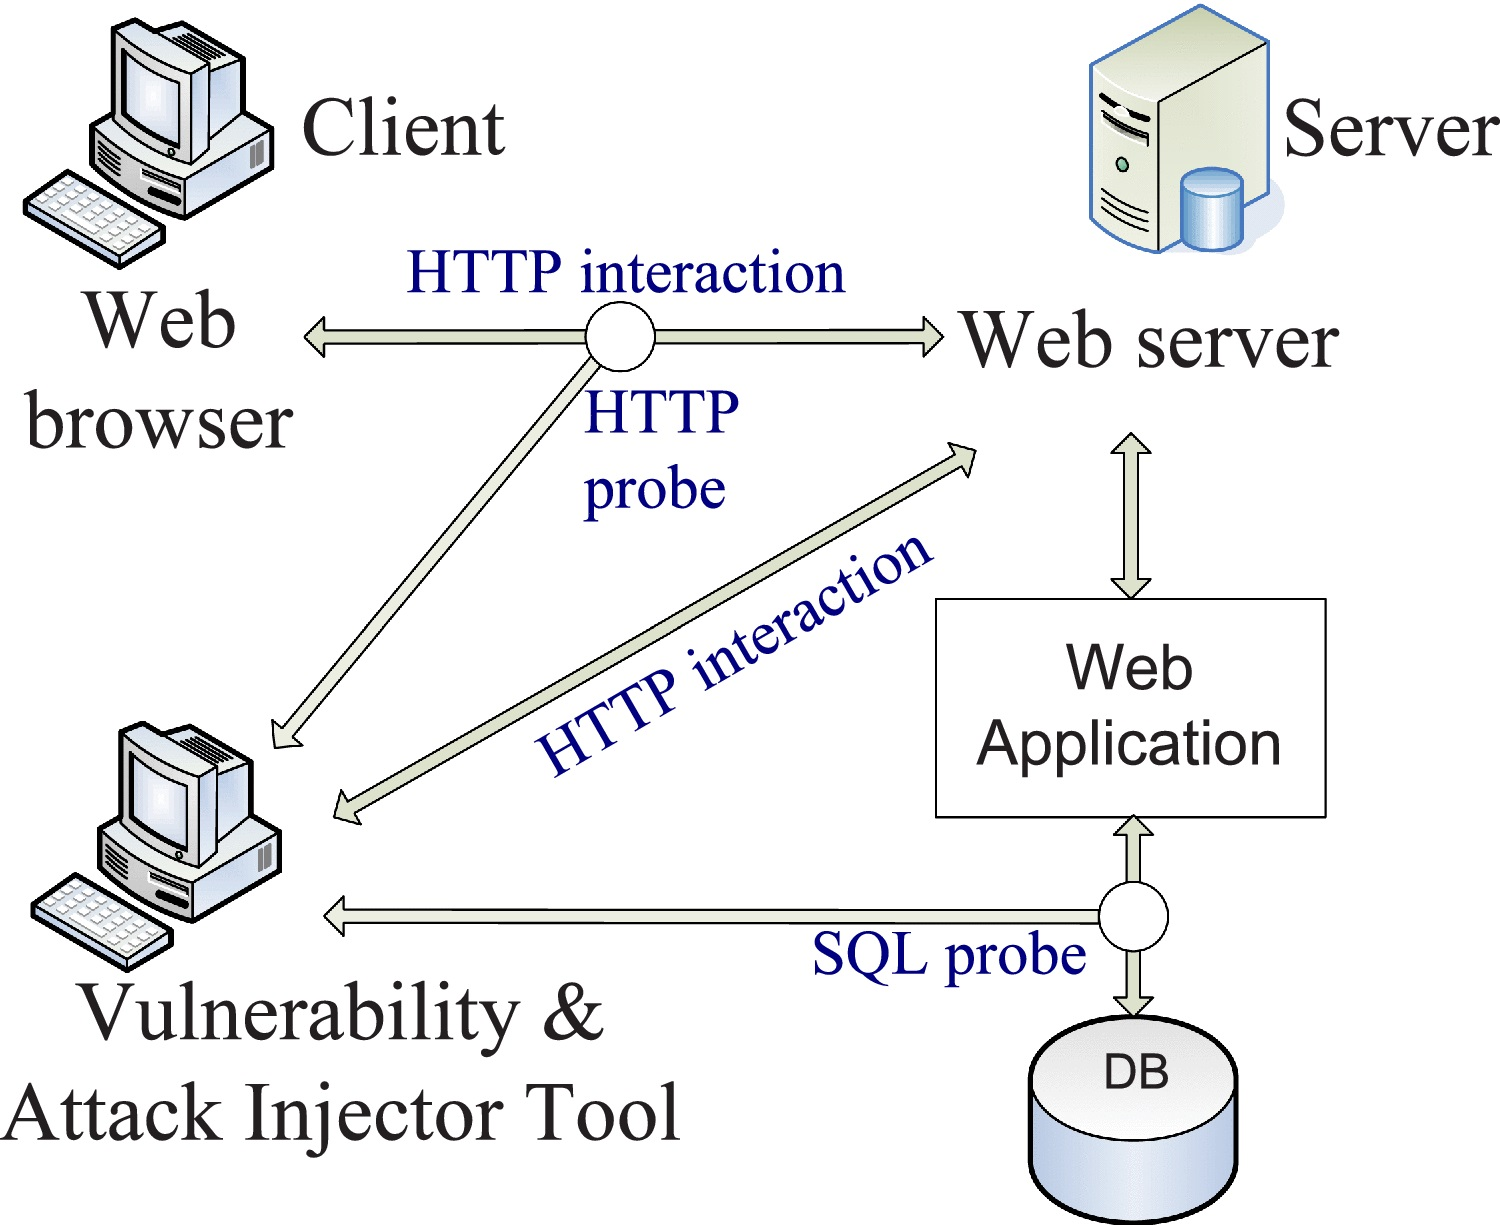
\includegraphics[width=0.5\textwidth]{figures/vait_setup.jpg}
	}
	\subfigure[Attack Injection Results of the Web Applications Analyzed]{\label{fig:web_evaluation_results}
		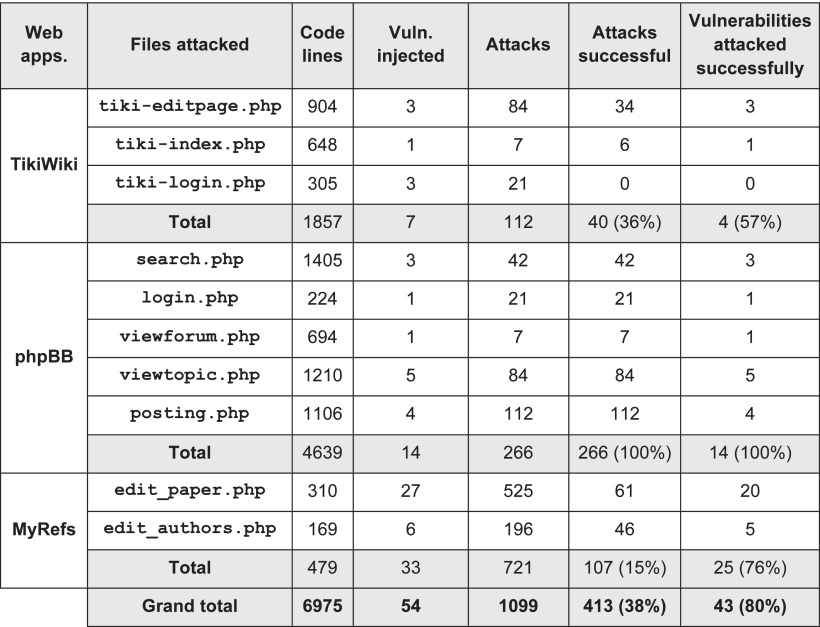
\includegraphics[width=0.5\textwidth]{figures/web_evaluation_results.jpg}
	}
	\caption{VAIT in a typical setup (a) and Attack Injection Results of the Web Applications Analyzed (b) \cite{6629992_Fronseca}.}
	\label{fig:vait}
\end{figure}
The automated attack of a web application is a multistage procedure that includes: preparation stage, vulnerability injection stage, attack load generation stage, and attack stage. The collection of information about the web application pages and their links can be done manually or using a web crawler for the preparation stage. In order to keep the same conditions for all the applications analyzed all the tests were done using the same web crawler (\textbf{Acunetix} web vulnerability scanner). Refer the Fig. \ref{fig:web_evaluation_results} for results of the security evaluation of target web applications. The tool took approximately 11 minutes in the attack stage of the TikiWiki, 12 minutes in the phpBB and 4 minutes in the MyReferences. The vulnerabilities injected represent all the "Missing Function Call Extended" SQLi types that can realistically be injected into the files used in the experiments. On average, the tool injected one vulnerability for every 129 lines of PHP code. Only 20 percent out of all the vulnerabilities injected could not be attacked. From the results its concluded that tool is effective in providing a sufficient number of realistic vulnerabilities in a web application and that these vulnerabilities can be successfully attacked. 

\subsection{Evaluation of Qualitative Methods}
The major advantages of qualitative method are it allows for putting in order risks according to priority, allows for determination of areas of greater risk in a short time and without bigger expenditures and analysis is relatively easy and cheap. However it does not allow for determination of probabilities and results using numerical measures and achieved results have general character, approximate etc.

\section{Quantitative Security Evaluation}\label{sec:quantitative}
'Quantitative' - means 'that is or may be estimated by quantity'. Quantitative security evaluation produces quantitative results which can be easily interpreted mathematically. Due to the similarities between security and dependability, the techniques for model-based techniques applied to the dependability domain has been adapted to evaluation of security. The difference is that dependability metrics measure the effect of natural or accidental failures whereas the security evaluation metrics measure the impact of intentional failures caused by attacks. A detailed discussion on the adaptation of model-based metrics from dependability to security is provided in [\citealp{1335467_Nicol}]. Dependability attributes include: \textbf{Reliability} - continuity of service , \textbf{Safety} - non-occurrence of catastrophic consequences, \textbf{Maintainability} - ability to undergo repairs and evolutions, \textbf{Availability} - readiness for usage, \textbf{Integrity} - data and programs are modified or destroyed only in a specified and authorized manner and \textbf{Confidentiality} - sensitive information is not disclosed to unauthorized recipients. Security evaluation is mainly concerned with primarily evaluating the last three attributes.

\subsection{Combinatorial methods}
These methods are used to evaluate system dependability measures. Reliability Block diagrams (RBD) and Fault Trees (FTs) are the typical combinatorial methods used in dependability analysis. These methods can be adapted to security domain like the method Attack Trees. 

\textbf{Attack Trees} are used to evaluate security of the system. Attack trees are closely related to fault trees, they consider the security breach as a failure and illustrates the group of events that can cause the system failure in a combinatorial way. Attack tree models all possible attacks against a system. Its a formal method which describes security of systems and subsystems based on numerous attacks. 

\textbf{Structure of an Attack Tree:} In attack trees the attacks of the systems are represented in the form a tree with root node represents the goal of attack and leaf nodes as the different ways to achieve the goal (atomic attacks). There are two kinds of root nodes AND nodes and OR nodes. An AND node represents an attack goal for which a set of subgoals (represented by leaf nodes) must be achieved in order for the attack to succeed. While an OR node represents an attack goal that can be achieved in several ways, which are represented by the OR node's children. Representation of an AND node OR node is given in Fig. \ref{fig:and_or_node}. As shown in figure in case of an AND node goal G$_0$ can be achieved if the attacker achieves each of G$_1$ through G$_n$ and in case of an OR node goal G$_0$S can be achieved if the attacker achieves any one of G$_1$ through G$_n$. 

\begin{figure}[h]
	\centering
	\subfigure[And node]{\label{fig:and_node}
		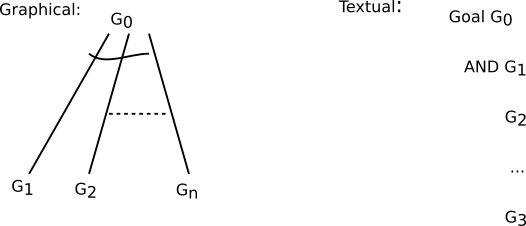
\includegraphics[width=0.5\textwidth]{figures/and_node.png}
	}
	\subfigure[OR node]{\label{fig:or_node}
		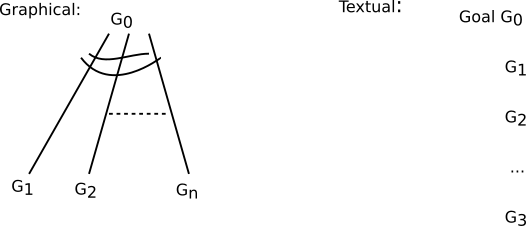
\includegraphics[width=0.5\textwidth]{figures/or_node.png}
	}
	\caption{AND node (a) and OR node (b) \cite{1335467_Nicol}.}
	\label{fig:and_or_node}
\end{figure}

\textbf{Evaluating Attack Trees:} The leaf nodes can take Boolean value(e.g., possible versus impossible attacks) or Continuous value (e.g., probability that the attack will succeed/fail). A node's value is a function of its children's values. If the assigned value is Boolean then AND node's value is the Boolean and of all values of its children and OR node's value is the Boolean or of all values of its children. When cost value is considered, the value of the AND node is the sum of the values of its children, and the value of the OR node is the minimum of the values of its children. The attack tree can be used to evaluate different aspects of the system security, depending on the kind of value that is assigned to the leaf nodes.

Attack trees thus help in providing a systematic ay to describe the security vulnerabilities and finally for the security assessment for making security decisions. The attack tree for a larger system can be modeled combining attack trees derived from different security features of the system.  

\subsection{State-Based Stochastic Methods}
In such models, the system is expressed as a finite state machine.  Each state of the system represents the security operational mode of the system. The states are modeled as one or more good states and one or more failure states. Good states are those in which the system is able to deliver the required services, even in the presence of attacks. Whereas, in security failure states, the system has been compromised by attacks in a way that its intended services can no longer be delivered. During the operation of the system continuously alternates between several possible states. A state transition is triggered by the appearance or remediation of a vulnerability i.e. the successful execution of an attack step or the responsive action performed by the security mechanism.

State-based metric models the system using Continuous-Time Markov Chain (CTMC) with discrete state space. CTMC is based on Markov property. As per Markov property, the probability distribution of the next state depends only on the current state and not on the previous states. Also, the time spent in each state takes a continuous set of values (i.e., non-negative real values), and follows an exponential distribution.

The major quantitative models based on stochastic models are described below.
\begin{enumerate}[(a)]
	\item {\textbf{Time-Based Security Metrics}\newline 
	Its based on the amount of time to make the system to be compromised by a successful attack. Larger the time value more secure the system is. One of the time based Metrics is based on Privilege Graphs.\\
    \textbf{Privilege Graph-Based Metrics}\newline 
	To evaluate system security the stated-based Markov model proposed by Dacier et al. \cite{Dacier1996QuantitativeAO} based on the Mean Time to Failure (MTTF) metric is being used. In their model with the help of a privilege graph the vulnerabilities of a system is represented. In this graph nodes represent the access rights (privileges) at hosts and arcs represent the actions that enable the transition from one privilege to another. Each arc is labeled with a value ($\lambda$) that represents the success rate of an elementary attack (privilege escalation). Once the privilege graph is constructed, it is turned into a CTMC containing all possible attack paths to target nodes. Refer Fig. \ref{fig:privilege_graph_example} for an example of a privilege graph.  The Markov model is based on the assumption that the success probability of an elementary attack before time t is represented by an exponential distribution given by: $P(t) = 1 - e^{-\lambda t}$. The mean time of succeeding in an elementary attack is given by $1/\lambda$. The MTTF of the system is computed by aggregating all the mean times necessary for succeeding in elementary attacks that lead to the targets.\\
		
	\begin{figure}[h]
		\centering
		\subfigure[1) X can guess Y's password; 2) X is in the Y's ".rhost"; 3) Y is a subset of X; 4) X can attack Y via Email; 5) Y uses a program owned by X; 6) X can modify a "setuid" program owned by Y.]
		{\label{fig:privilege_graph}
			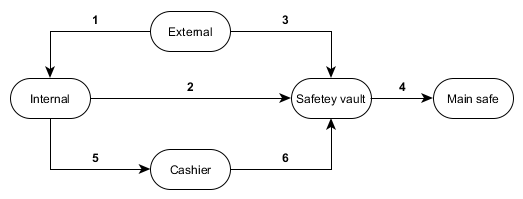
\includegraphics[width=0.8\textwidth]{figures/privilege_graph.png}
		}
		\caption{Example of a privilege graph \cite{Dacier1996QuantitativeAO}.}
		\label{fig:privilege_graph_example}
	\end{figure}
		
	Even though MTTF provide useful security level information, they do not take into account of partial or interrupted attacks (which can also cause damage to the system).}

	\item {\textbf{Probability-Based Security Metrics}\newline 
	Probability-based security metrics normally express the likelihood of a threat compromising the system or the probability that the system is secure.\\
	
 	Li et al. \cite{4695835_Li} presents a renewal stochastic model to estimate the likelihood that an adversary exploits a randomly selected system vulnerability. This likelihood is given by the q metric namely the probability that a randomly picked vertex is compromised when the system enters its steady state. A lower q value indicates more security. To compute q, the network is represented as a vulnerability graph, in which every node represents a vulnerability, and the arc or the edge shows that the exploitation of one vulnerability could lead to the exploitation of the other. At any given instant of time, each node can either be in a secure state or a compromised state. The behavior of the nodes is described by a series of random variables that represent compromise rates and fix rates. Refer Fig. \ref{fig:probablistic_sec_mod} for a probability security model.}
 	\begin{figure}[h]
 		\centering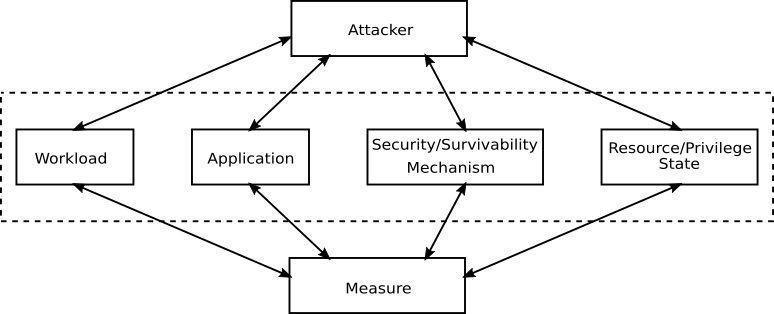
\includegraphics[width=0.8\textwidth]{figures/probablistic_sec_mod.png}
 		\caption{Probabilistic security model structure \cite{1335467_Nicol}.}
 		\label{fig:probablistic_sec_mod}
 	\end{figure}
\end{enumerate}

\subsection{Attack Graphs}  
Attack graphs depict ways in which an adversary can exploit vulnerabilities to break into a system. Attack graph can be automatically to generate attack paths to analyze the network vulnerability. It can show users the weak point in the network analysis process for network security risk analysis. Once a potential attack path is found, attack graph tools can generate attack graph or attack trees to help system administrators understand how attacks happen, and then take defensive measures. There are many tools to automatically build attack graphs for a given network. For example open source tools like MulVAL, TVA. Attack Graph Toolkit, NetSPA and the commercial tools like Cauldron, FireMon, Skybox View.

The major quantitative models based on attack graphs are described below.
\begin{enumerate}
	\item {\textbf{Path Metrics}\newline 
		Its based on the characteristics of the attack paths. One of the path metrics is Shortest Path Metric (SP) proposed by Phillips and Swiler \cite{CynthiaPhillips1998}. As per this metric, the network is modeled as a condition-oriented network graph and security level corresponds to the length of the smallest attack path that an adversary can take to reach the desired goal state(compromised state). So longer the shortest path, more secure the network. The advantage of SP metric is simplicity however it does not take into account for the number of different shortest paths in a network. To overcome this researchers have come up with different path metrics like Number of Paths metric (NP), Mean of Path Lengths metric (MPL).}
	
	\item {\textbf{Non-Path Metrics}\newline 
		Its based on the number of hosts that can be compromised. Pamula et al. \cite{J.Pamula2006} propose the Weakest Adversary metric, which is based on a condition-exploit-oriented attack graph.
		This metric illustrates the security strength of a network by means of the least amount of effort an attacker needs to compromise a given network asset. The authors consider the minimum effort expended by an attacker as the strength of the set of initial conditions (of an attack graph) that enable the compromise of a network. Therefore, when comparing two networks, the less secure network will be the one with the weaker set of initial conditions.}
	
	\item {\textbf{Probabilistic Metrics}\newline
		Probabilistic AG-based metrics either take probability values as input, or produce probability values as output, or both. The two common Probabilistic metrics are PageRank-Based Metric :  This metric measures the probability of goal states occurring	(i.e., probability of the network being compromised) and Metric based on Independent Attack Paths : Uses an exploit dependency graph to quantify network security by propagating exploit likelihood scores from initial exploit to final exploit(compromised state).}
	
		\item {\textbf{Bayesian Network Based Metrics}\newline
		A Bayesian Network (BN), also known as belief network, can be defined as a directed acyclic graph (DAG) with nodes representing variables of a system and edges representing causal relationships among these variables. In BN each node is assigned with Conditional Probability Table (CPT). Theses values indicate the conditional probabilities of each vulnerability being exploited.
		}
\end{enumerate}

\subsection{Common Vulnerability Scoring System}
The Common Vulnerability Scoring System (CVSS) is a frame work used to quantify the severity and risk of a vulnerability to an information asset in a computing environment.It was designed by NIST (National Institute of Standard and Technology) and a team of industry partners. A CVSS score is a decimal number in the range from 1 to 10. The security experts assign set of quality values to predefined attributes of given vulnerability and CVSS score for the desired vulnerability is calculated using the same. For every qualitative value of a given attribute has a predefined corresponding quantitative value. Using these quantitative values final CVSS score is calculated. The more vulnerabilities a software product has, the lower level of trustworthiness this software product has. The more severe vulnerabilities a software product has, the less secure this software will be.CVSS metrics for vulnerabilities are divided into three groups: Base metrics measure the intrinsic and fundamental characteristics of vulnerabilities that do not change over time or in different environments. Temporal metrics measure those attributes of vulnerabilities that change over time but do not change among user environments. Environmental metrics measure those vulnerability characteristics that are relevant and unique to a particular user's environment. Now a days Several vulnerability databases use CVSS to quantify the severity of reported vulnerabilities.

In the paper, \cite{Wang:2009:SMS:1566445.1566509} applied CVSS to find out the security metrics for the software products. They had applied the derived security metrics formula for the Internet applications such as Mozilla Firefox 2, Microsoft Internet Explorer 6  and Microsoft Internet Explorer 7 to find out their vulnerabilty scores and finally the security metric. The final security metric scores for applications were Mozilla Firefox 2 = 6.7, Microsoft Internet Explorer 6 = 8.7 and Internet Explorer 7 = 7.9. 

\subsection{Evaluation of Quantitative Methods}
The major advantages of these methods are they allow for definition of consequences of incidents occurrence in quantitative way, what facilitates realization of costs and benefits analysis during selection of protections and they give more accurate image of risk. However quantitative measures depend on the scope and accuracy of defines measurement scale, results of analysis may be not precise and even confusing and these methods are generally more expensive, demanding greater experience and advanced tools.
	
\section{Conclusions}\label{sec:conclusions}
In this paper detailed analysis of security evaluation is presented. Qualitative and Quantitative security evaluation methods are discussed. Qualitative security evaluation methods are focused on detection and prevention of vulnerabilities while the Quantitative methods provide a characterization of security risks in terms of vulnerabilities present in the software. Such characterization of vulnerabilities can provide us metrics that can be used by the developers and potential users. Results of these evaluation methods are useful in developing guidelines for allocation of resources for security testing, scheduling, and development of security patches. Furthermore, it can be used by the users for assessing risk and estimating needed redundancy in resources and procedures to handle potential breaches. Security evaluation can be useful to know existing threats and potential vulnerabilities of your system, e.g., to avoid them in future systems. 

In this survey only a few of the security evaluation methods are discussed. But there are so many security evaluation methods available and the major challenge would be choosing the right security evaluation method for the corresponding software system. This is often a difficult task. Usually for the security evaluation of software systems (Web applications, Network management) different security evaluation methods are applied, their results are compared and the best among them is chosen. In case complex systems several methods are combined to produce a better result. This makes the job of the security expert challenging. The area of security evaluation is growing rapidly and lately even machine learning concepts are used for the same.  

\bibliography{template}

\end{document}
